%\thispagestyle{myheadings}
\section{Invited Talk: Sharon Goldwater}
\index{Goldwater, Sharon}

\begin{center}
\begin{Large}
{\bfseries\Large Towards more universal language technology: unsupervised learning from speech}\vspace{1em}\par
\end{Large}

%% \begin{center}
%%   \begin{tabular}{m{1in}b{1in}}
%%     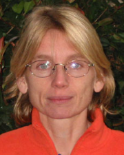
\includegraphics[width=1in]{content/monday/cortes-headshot.png}
%%     & {\bfseries Corinna Cortes} \newline Google Research, NY
%%   \end{tabular}
%% \end{center}

\daydateyear, 9:00--10:00 \vspace{1em}\\
\PlenaryLoc \\
\vspace{1em}\par
%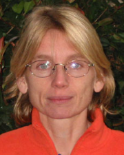
\includegraphics[height=100px]{content/monday/cortes-headshot.png}
\end{center}

\noindent
{\bfseries Abstract:} Speech and language processing has advanced enormously in the last
        decade, with successful applications in machine translation,
        voice-activated search, and even language-enabled personal
        assistants. Yet these systems typically still rely on learning from
        very large quantities of human-annotated data. These
        resource-intensive methods mean that effective technology is available
        for only a tiny fraction of the world's 7000 or so languages, mainly
        those spoken in large rich countries.
        
        This talk describes our recent work on developing \textit{unsupervised}
        speech technology, where transcripts and pronunciation dictionaries
        are not used. The work is inspired by considering both how young
        infants may begin to acquire the sounds and words of their language,
        and how we might develop systems to help linguists analyze and
        document endangered languages. I will first present work on learning
        from speech audio alone, where the system must learn to segment the
        speech stream into word tokens and cluster repeated instances of the
        same word together to learn a lexicon of vocabulary items. The
        approach combines Bayesian and neural network methods to address
        learning at the word and sub-word levels.

\vspace{3em}\par 

\vfill
\noindent

{\bfseries Biography:} Sharon Goldwater is a Reader at the University of Edinburgh's
  School of Informatics, where she is a member of the Institute for
  Language, Cognition and Computation. She received her PhD in 2007
  from Brown University and spent two years as a postdoctoral
  researcher at Stanford University before moving to Edinburgh. Her
  research interests include unsupervised learning for speech and
  language processing, computer modelling of language acquisition
  in children, and computational studies of language
  use. Dr. Goldwater co-chaired the 2014 Conference of the European
  Chapter of the Association for Computational Linguistics and is
  Chair-Elect of EACL. She has served on the editorial boards of
  the Transactions of the Association for Computational
  Linguistics, the Computational Linguistics journal, and OPEN
  MIND: Advances in Cognitive Science (a new open-access
  journal). In 2016, she received the Roger Needham Award from the
  British Computer Society, awarded for "distinguished research
  contribution in computer science by a UK-based researcher who has
  completed up to 10 years of post-doctoral research."
\newpage
